\chapter{Methodological Contribution}
\label{cap:contrib}

This chapter is devoted to analyzing which parts of the project are of deep importance, such as the distribution of the data or which hyperparameters must be taken into account for training, and to designing a diagram or solution that provides answers to these matters. In this chapter, we also examine the reasons behind the selection of the base model for transfer learning and the methods used to regularize these trained models.

\section{Data Analysis}
\label{sec:data-analysis}

As previously mentioned, the data is acquired from the ISIC Archive, specifically from the SIIM-ISIC Melanoma Classification competition available on Kaggle \cite{ISICKaggle}. This challenge's dataset is a subset of the larger ISIC Archive and includes data from 2019 and 2020. \\

For the thesis, we opted to use images with a resolution of 512x512 pixels, despite the availability of higher resolutions such as 768x768 and 1024x1024. The decision to select a lower resolution was purely technical, as higher resolution images would require greater computational resources. \\

For training the models, we utilized 8 classes selected from the original set, as the remaining classes were considered residuals. Any samples that were not categorized as one of the following classes were excluded from the training process. \\

\begin{itemize}
    \item melanoma
    \item nevus
    \item BCC (Basal Cell Carcinoma)
    \item BKL (Benign lesions of the keratosis)
    \item AK (Actinic Keratosis)
    \item SCC (Squamous Cell Carcinoma)
    \item VASC (Vascular Lesions)
    \item DF (Dermatofibroma)
\end{itemize}

The filtered dataset consists of 31,265 different image samples with an unbalanced distribution across all classes (see \textit{Figure \ref{fig:hole-dataset-distribution}}).

\begin{figure}[H]
\centering
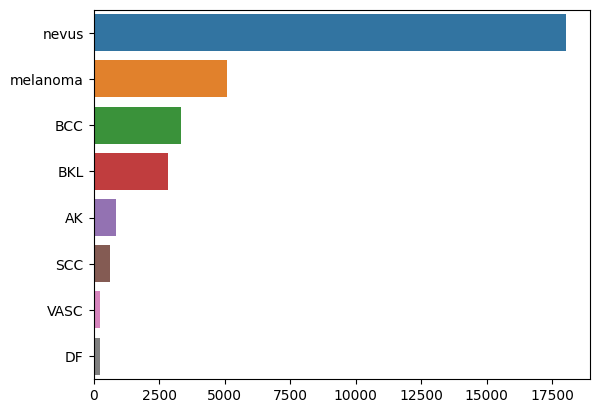
\includegraphics[width=0.9\textwidth]{imatges/methodological_contribution/hole-dataset-diagnosis.png}
\caption[Filtered Dataset Distribution]{\textit{Filtered Dataset Distribution. Having an unbalanced dataset is challenging during training. Models tend to overfit to the more frequent classes since targeting the majority class is easier. Illustration by Author}}
{\label{fig:hole-dataset-distribution}}
\end{figure}

\section{Stratification}

Unbalanced datasets present a significant challenge in machine learning problems. Various methods can be employed to address this issue, including over-sampling, under-sampling, and more. In our approach, we decided to tackle this problem by utilizing stratification in the train, validate, and test datasets. This ensures that all datasets maintain the same distribution of classes, even though they are unbalanced. \\

To address the issue of unbalanced distribution, we created a function that made use of the {\tt stratify} parameter in the scikit-learn's {\tt train\_test\_split} function, which is designed for such scenarios. By default, this parameter is set to the labeled prediction, ensuring that the resulting train, validate and test datasets maintain a proportional representation of the different classes in the data.

\begin{Verbatim}[fontsize=\scriptsize]
def train_validate_split(df: pd.DataFrame,
                         random_state: int = 42,
                         validate_size: int = 0.25):
    """Split dataframe into random train and validate dataframe,
    it uses stratify thecnique because of the unbalanced dataset"""

    X_train, X_val = train_test_split(df,
                                      random_state=random_state,
                                      train_size=(1-validate_size),
                                      stratify=df['target'])
    X_train = pd.DataFrame(X_train)
    X_train.columns = df.columns
    X_val = pd.DataFrame(X_val)
    X_val.columns = df.columns

    return X_train, X_val
\end{Verbatim}

Creating the train, validation and test dataset was as easy as follow,

\begin{Verbatim}[fontsize=\scriptsize]
train_df, validate_df = m_dataset.train_validate_split(df,
                                                       random_state=42,
                                                       validate_size=0.2)

validate_df, test_df = m_dataset.train_validate_split(validate_df,
                                                      random_state=42,
                                                      validate_size=0.5)
\end{Verbatim}

Note that the training dataset comprises 80\% of the filtered dataset, which corresponds to a total of 25,012 samples. In contrast, both the validation and test datasets are composed of 10\% of the filtered dataset, amounting to 3,126 samples each.

\section{Data Augmentation}

As it was explained in \textit{Chapter \ref{cap:prelim}}, data augmentation is a technique that
creates more data by applying multiple transformations on an image. The  main goal of data augmentation is to increase the volume, quality and diversity of training data. \\

For the thesis, the python package {\tt albumentations} was used for this goal,
the package support a big variety of transformations, some of these transformations are
represented bellow.

\newpage

\textbf{Horizontal and vertical flips} \\

    An image flip means reversing the rows or columns of pixels in the case of a vertical or horizontal flip respectively.

    \begin{figure}[H]
    \centering
    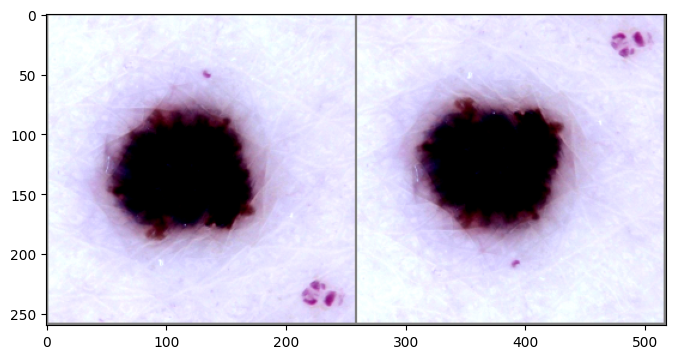
\includegraphics[width=0.6\textwidth]{imatges/methodological_contribution/horizontal-flip.png}
    \caption[Horizontal Flip]{\textit{Horizontal flip. \textbf{Left}: original image, \textbf{Right}: augmented image. Illustration by Author}}
    \end{figure}

\vspace{0.5cm}
\textbf{Gaussian blur} \\

Blur the input image using a Gaussian filter with a random kernel size.

    \begin{figure}[H]
    \centering
    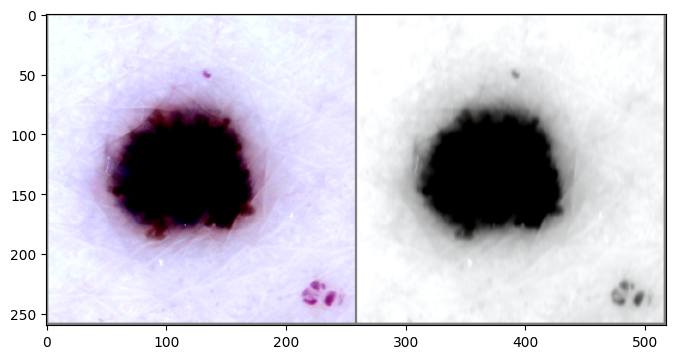
\includegraphics[width=0.6\textwidth]{imatges/methodological_contribution/gaussianblur.png}
    \caption[Gaussian Blur]{\textit{Gaussian Blur. \textbf{Left}: original image, \textbf{Right}: augmented image. Illustration by Author}}
    \end{figure}

\newpage

\textbf{Random brightness contrast} \\

Randomly change brightness and contrast of the input image.

    \begin{figure}[H]
    \centering
    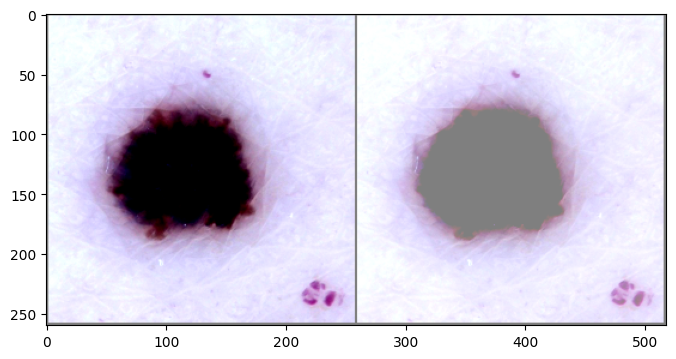
\includegraphics[width=0.6\textwidth]{imatges/methodological_contribution/random-brigness-constrast.png}
    \caption[Random Brightness Contrast]{\textit{Random Brightness Contrast. \textbf{Left}: original image, \textbf{Right}: augmented image. Illustration by Author}}
    \end{figure}

As a result of applying the following data augmentation pipeline,

\begin{Verbatim}[fontsize=\scriptsize]
    transforms_train = A.Compose([
        A.Transpose(p=0.5),
        A.VerticalFlip(p=0.5),
        A.HorizontalFlip(p=0.5),
        A.RandomBrightnessContrast(contrast_limit=0.2, p=0.75),
        A.OneOf([
            A.MotionBlur(blur_limit=5),
            A.MedianBlur(blur_limit=5),
            A.GaussianBlur(blur_limit=5),
            A.GaussNoise(var_limit=(5.0, 30.0)),
        ], p=0.7),
        A.OneOf([
            A.OpticalDistortion(distort_limit=1.0),
            A.GridDistortion(num_steps=5, distort_limit=1.),
            A.ElasticTransform(alpha=3),
        ], p=0.7),
        A.CLAHE(clip_limit=4.0, p=0.7),
        A.HueSaturationValue(hue_shift_limit=10,
                             sat_shift_limit=20,
                             val_shift_limit=10,
                             p=0.5),
        A.ShiftScaleRotate(shift_limit=0.1,
                           scale_limit=0.1,
                           rotate_limit=15,
                           border_mode=0,
                           p=0.85),
        A.Resize(image_size, image_size),
        A.CoarseDropout(max_holes=1,
                        max_height=int(image_size * 0.375),
                        max_width=int(image_size * 0.375),
                        p=0.7),
        A.Normalize(mean=mean, std=std)
    ])
\end{Verbatim}

The train dataset (\textit{Figure \ref{fig:sample-of-datasets}}),

\begin{figure}[H]
\centering
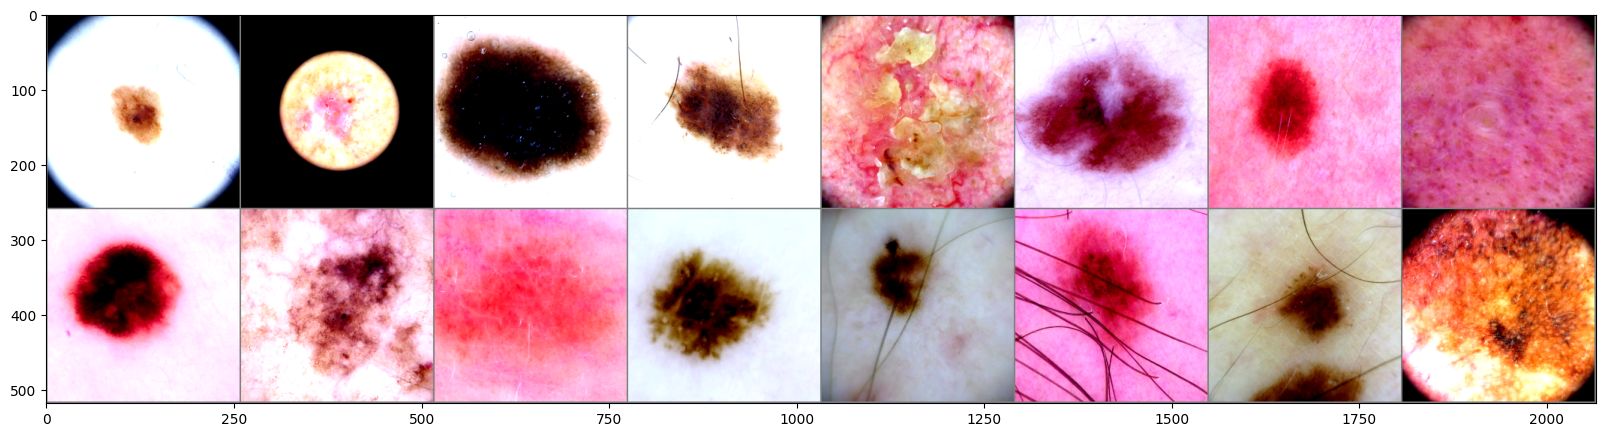
\includegraphics[width=\textwidth]{imatges/methodological_contribution/random-sample-of-isic.png}
\caption[Random sample of images in the train dataset]{\textit{Random sample of images in the train dataset. Illustration by Author}}
{\label{fig:sample-of-datasets}}
\end{figure}

Is mapped into an augmented train dataset (\textit{Figure \ref{fig:aug-sample-of-datasets}}).

\begin{figure}[H]
\centering
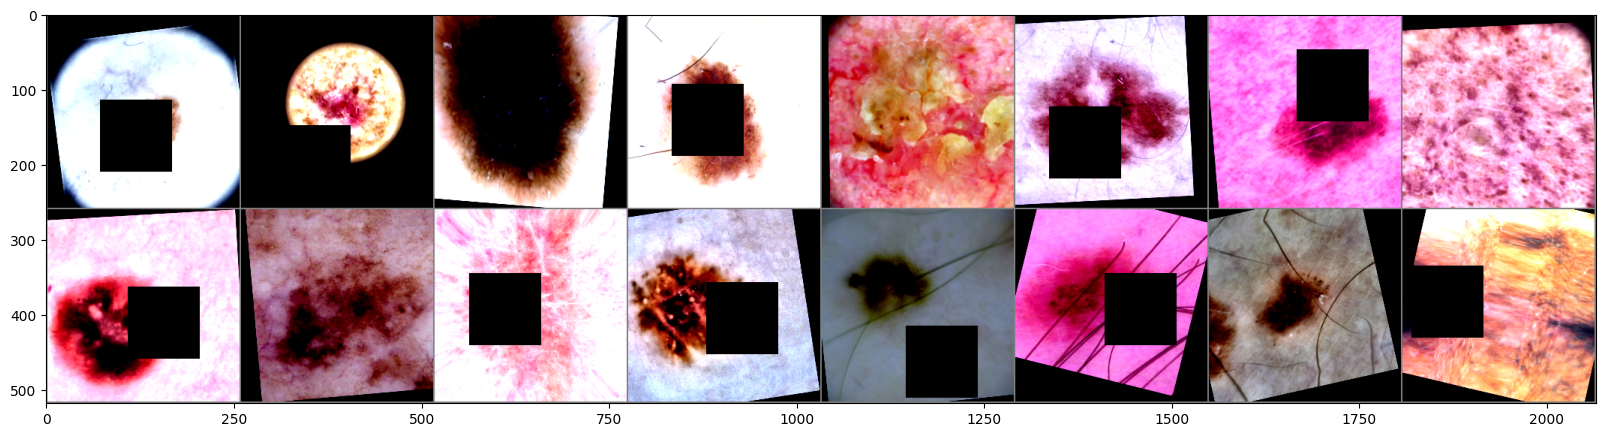
\includegraphics[width=\textwidth]{imatges/methodological_contribution/random-sample-of-isic-augmented.png}
\caption[Augmented random sample of images in the train dataset]{\textit{Augmented random sample of images in the train dataset. Illustration by Author}}
{\label{fig:aug-sample-of-datasets}}
\end{figure}

\newpage

\section{ResNet-18}

We utilized the pre-trained weights of the {\tt ResNet-18} as the base model for transfer learning. As described in \textit{Chapter \ref{cap:prelim}}, this model achieves an accuracy of approximately 69.76\% on the {\tt ImageNet} dataset, which may not be as high as some other models. However, due to its relatively small number of trainable parameters (11.7 million), we decided to select this model over other available options. \\

In ResNet architecture (Figure \ref{fig:resnet-18-arch}), each layer of the network contains a residual block (BasicBlock).

\begin{figure}[H]
\begin{adjustbox}{width=\textwidth, trim={0.2cm 0pt 1.5cm 0pt}, clip}
\centering
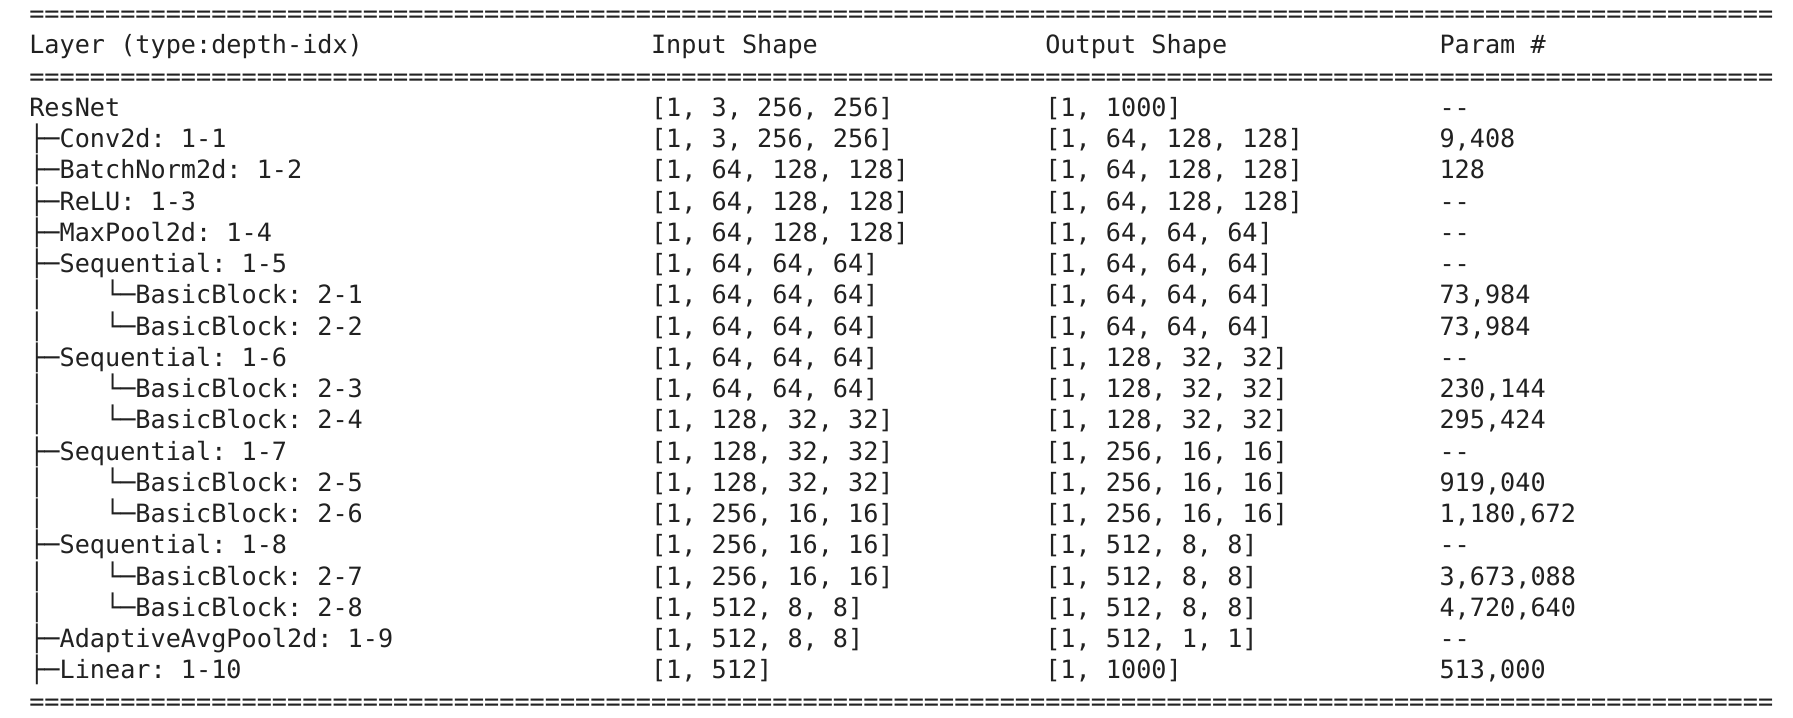
\includegraphics[width=\textwidth]{imatges/methodological_contribution/residual-blocks.png}
\end{adjustbox}
\caption[Resume of the ResNet-18 Architecture]{\textit{Resume of the ResNet-18 Architecture. Notice that the default output dimension of ResNet-18 is 1000. Illustration by Author}}
{\label{fig:resnet-18-arch}}
\end{figure}

A residual block
consists of multiple convolutional layers followed by batch normalization and
activation functions (\textit{Figure \ref{fig:resnet-18-residual-block}}).

\begin{figure}[H]
%\begin{adjustbox}{width=\textwidth, trim={0.2cm 0pt 1.5cm 0pt}, clip}
\centering
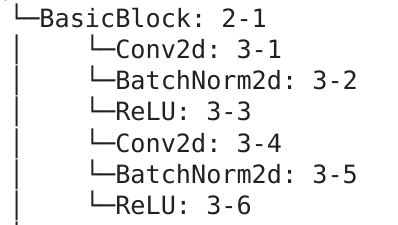
\includegraphics[width=0.4\textwidth]{imatges/methodological_contribution/basic-block.png}
%\end{adjustbox}
\caption[ResNet18 Residual Block]{\textit{ResNet18 Residual Block. Illustration by Author}}
{\label{fig:resnet-18-residual-block}}
\end{figure}

The input to a residual block is added to its output through
a skip connection, which directly connects the input to the output (\textit{Figure \ref{fig:skip-connection}}). This allows
the network to learn the residual information, or the difference between the
input and the desired output, making it easier for the network to learn the un-
derlying mapping.

\begin{figure}[H]
%\begin{adjustbox}{width=\textwidth, trim={0.2cm 0pt 1.5cm 0pt}, clip}
\centering
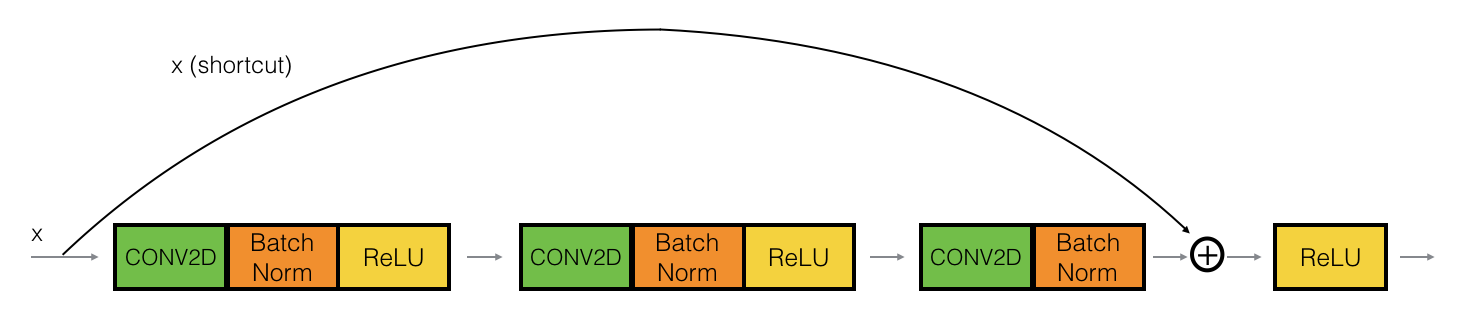
\includegraphics[width=\textwidth]{imatges/methodological_contribution/skip-connections.png}
%\end{adjustbox}
\caption[ResNet Skip Connection]{\textit{ResNet Skip Connection. Illustration by medium}}
{\label{fig:skip-connection}}
\end{figure}

There are many ways to use {\tt ResNet-18} as base transfer learning models. We made use of the PyTorch API to accomplish it.

\begin{Verbatim}[fontsize=\scriptsize]
from torchvision.models import (resnet18,
                                ResNet18_Weights)
net = resnet18(weights=ResNet18_Weights.IMAGENET1K_V1)
\end{Verbatim}

\section{Proposed Models}

As explained in the section before, the base model is the {\tt ResNet-18}. This model classify
between 1000 classes. But our goal is to classify between 8 different classes. \\

The very first approach to solve this issue was to encapsulate the ResNet into a {\tt Module} class, which is a class that can be trained in the PyTorch framework.

\begin{Verbatim}[fontsize=\scriptsize]
class ResNet18_Melanoma(nn.Module):

    def __init__(self, out_features: int):
        super(ResNet18_Melanoma, self).__init__()

        self.net = resnet18(weights=ResNet18_Weights.IMAGENET1K_V1)
        in_features = self.net.fc.in_features
        self.net.fc = nn.Identity()
        self.myfc = nn.Linear(in_features, out_features)

    def transfer(self, x: torch.Tensor):
        return self.net(x)

    def forward(self, x: torch.Tensor):
        x = self.transfer(x).squeeze(-1).squeeze(-1)
        x = self.myfc(x)
        return x
\end{Verbatim}

As you can see above, we utilize the weights of the trained {\tt ResNet-18} and save the trained model into an instance of the {\tt ResNet18\_Melanoma} class. Then, we retrieve the instance of the {\tt ResNet-18} and modify its fully connected layer by assigning it to an Identity layer, which doesn't perform any operations. Finally, we instantiate a new fully connected layer with the expected output size. In this case, the expected output size is 8, representing the number of classes. See \textit{Figure \ref{fig:resnet-18-melanoma-arch}}.

\begin{figure}[H]
\centering
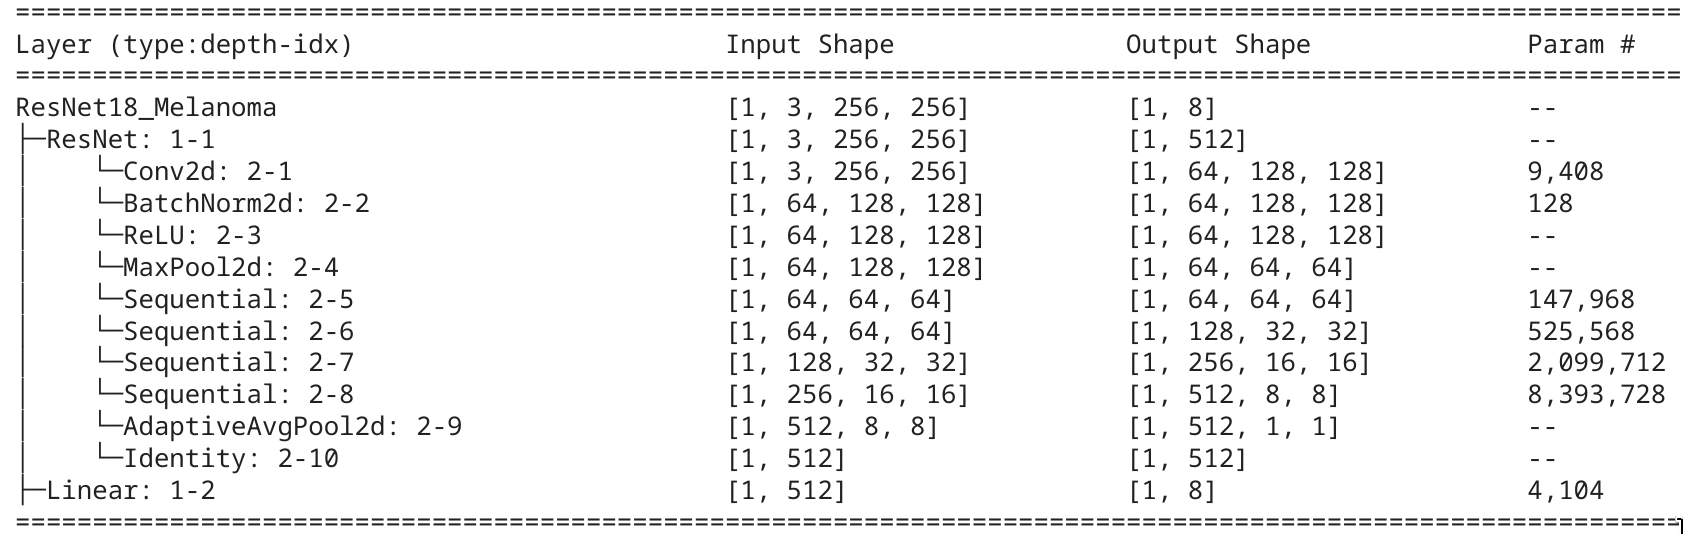
\includegraphics[width=\textwidth]{imatges/methodological_contribution/ResNet18_Melanoma.png}
\caption[Resume of the ResNet18\_Melanoma Architecture]{\textit{Resume of the ResNet18\_Melanoma Architecture. Notice that the output dimension of ResNet18\_Melanoma is 8. Illustration by Author}}
{\label{fig:resnet-18-melanoma-arch}}
\end{figure}


During the model training process, the {\tt forward} function is triggered with images represented as a tensor. It first performs transfer learning using the base model through the transfer function. Then, it utilizes the output of the transfer process to train the new fully connected layer. \\

In the evaluation and analyse stage of the different training approaches of the {\tt ResNet18\_Melanoma} we observed significant over-fitting. To address this issue, we propose the {\tt ResNet18\_Dropout\_Melanoma} model, which follows the same behavior as the previous model but includes a regularization layer that utilizes the average of 5 dropout layers after the transfer learning process. This regularization layer helps to mitigate the over-fitting problem found in the previous model.

\begin{Verbatim}[fontsize=\scriptsize]
class ResNet18_Dropout_Melanoma(nn.Module):
    """This model is based on ResNet18 but uses the
    average of the result of a list of dropout layers
    to avoid overfitting"""

    def __init__(self, out_features: int):
        super(ResNet18_Dropout_Melanoma, self).__init__()

        self.net = resnet18(weights=ResNet18_Weights.IMAGENET1K_V1)
        in_features = self.net.fc.in_features
        self.net.fc = nn.Identity()
        self.myfc = nn.Linear(in_features, out_features)
        self.dropouts = nn.ModuleList([nn.Dropout(0.5) for _ in range(5)])

    def transfer(self, x: torch.Tensor):
        return self.net(x)

    def forward(self, x: torch.Tensor):
        x = self.transfer(x).squeeze(-1).squeeze(-1)

        for i, dropout in enumerate(self.dropouts):
            if i == 0:
                out = self.myfc(dropout(x))
            else:
                out += self.myfc(dropout(x))

        out /= len(self.dropouts)
        return out
\end{Verbatim}

We provide the resume architecture of {\tt ResNet18\_Dropout\_Melanoma} model in \textit{Figure \ref{fig:resnet-18-dropout-melanoma-arch}}.
The {\tt recursive} label in the provided image means that the layers have been "forwarded" multiple times instead of constructed multiple times.

\begin{figure}[H]
\centering
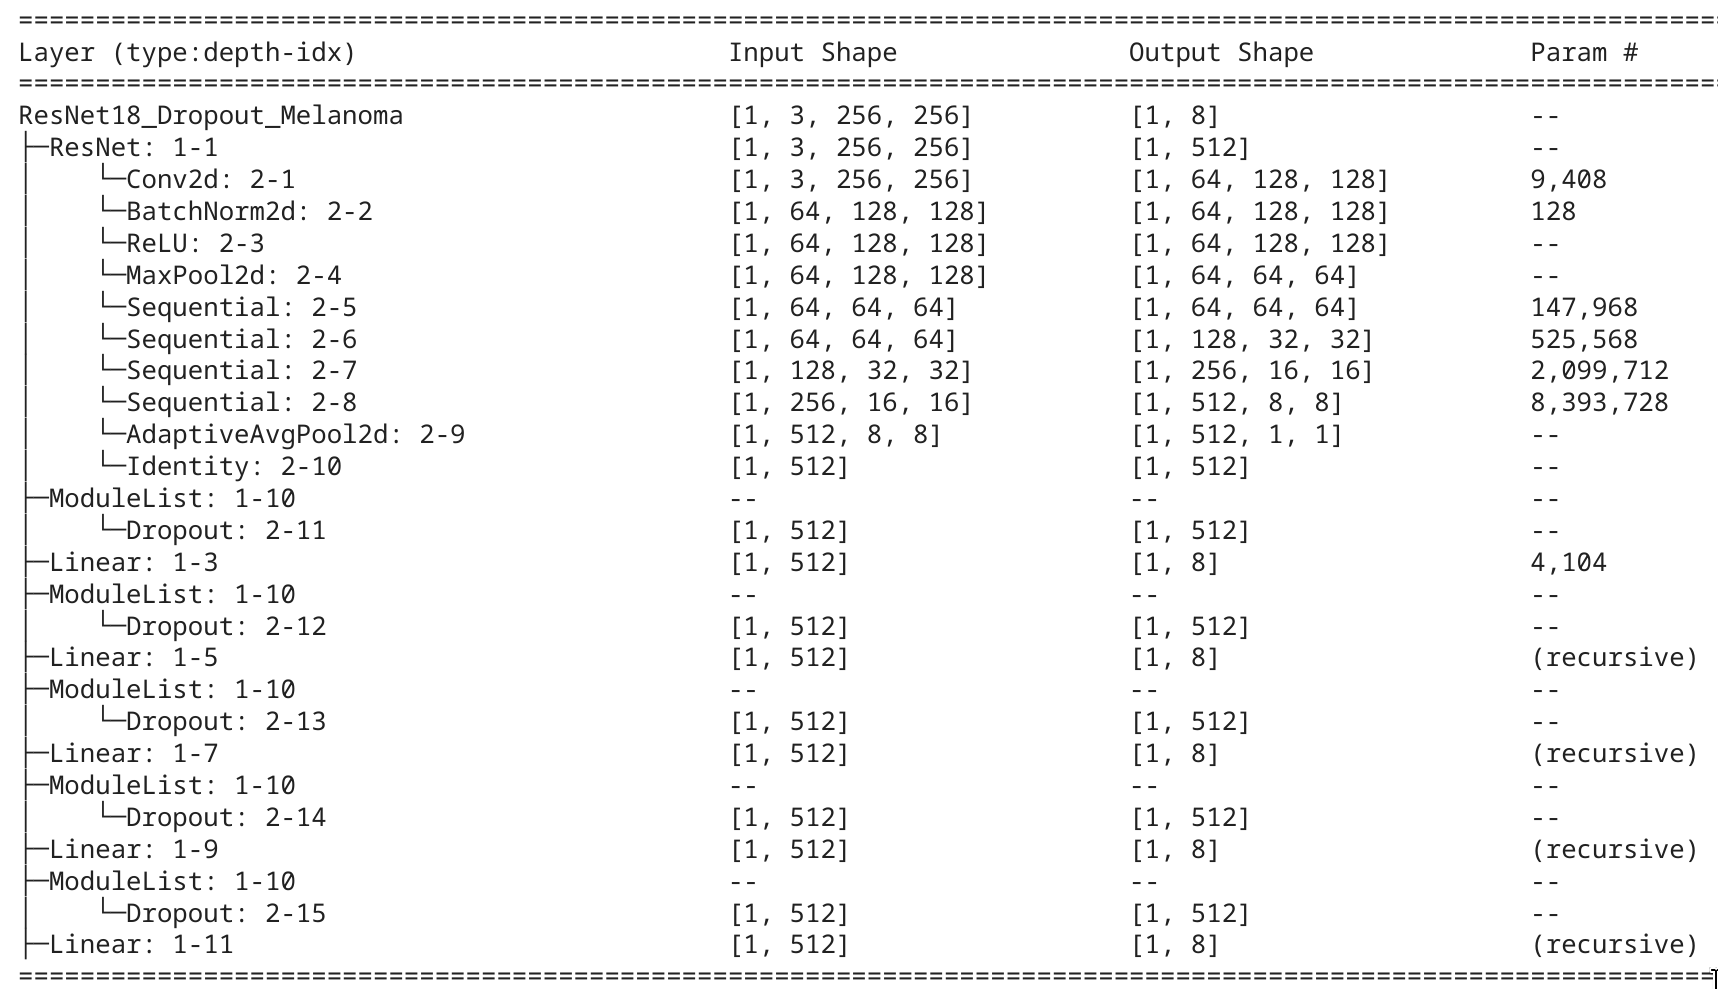
\includegraphics[width=\textwidth]{imatges/methodological_contribution/ResNet18_Dropout_Melanoma.png}
\caption[Resume of the ResNet18\_Dropout\_Melanoma Architecture]{\textit{Resume of the ResNet18\_Dropout\_Melanoma Architecture. Notice that the output dimension of ResNet18\_Dropout\_Melanoma is 8. Illustration by Author}}
{\label{fig:resnet-18-dropout-melanoma-arch}}
\end{figure}

You can instantiate any of these models with the necessary {\tt out\_features} by following the code snippet below:

\begin{Verbatim}[fontsize=\scriptsize]
out_features = len(mapping)
model = m_models.ResNet18_Dropout_Melanoma(out_features)
\end{Verbatim}

Note that the variable {\tt out\_features} should be defined before doing any instance.

\section{Train-Validate Loop}

\begin{Verbatim}[fontsize=\scriptsize]
def train_model(model: nn.Module,
                mel_idx: int,
                about_data: Dict,
                device: torch.device,
                criterion: nn.Module,
                optimizer: torch.optim.Optimizer,
                scheduler: torch.optim.lr_scheduler.LRScheduler = None,
                num_epochs: int = 25,
                patience: int = 5,
                writter: Writter = None,
                val_times: int = 1):
. . .
\end{Verbatim}

Among other features, the train validate loop supports:

\begin{itemize}
    \item Train the model using the training dataset.
    \item Validate the model using the validation dataset.
    \item Modify the optimizer's behavior using a scheduler.
    \item Implement an early stop mechanism by defining the {\tt patience} argument.
    \item Save the weights of the trained model and evaluate metrics using a higher-order function.
    \item Apply test-time augmentation during the validation phase, repeating it a certain number of times using the {\tt val\_times} argument.
\end{itemize}

\section{Writer Callback}

PyTorch does not provide built-in wrappers to automatically save model performance during the training and validation phases. However, it is essential to have information on how well a model performs after each epoch in order to compare different training approaches. \\

To address this issue, we have implemented a function that can save the model weights after each epoch and maintain a history of metrics from both the training and validation phases. Additionally, we log the training process by sending the latest state of the metrics using the Weight and Biases MLOPS service. This allows us to track and analyze the training progress effectively

\begin{Verbatim}[fontsize=\scriptsize]
def model_writter(model_name: str):
    """Saves the pythorch trainned model and generates
    a log file in csv format with the current trainning
    and validation phases. It finally send the last log
    to wand service."""

    def writter(point: Dict):
        # Save checkpoint
        m_checkpoint.save_checkpoint(point,
                                     model_name + '.pth.tar')

        # Logging the trainning
        log_filename = model_name + '.csv'
        stats = point['stats']
        pd.DataFrame(stats).to_csv(log_filename)

        # wand logging
        wandb.log({
            "train_acc": stats["train_acc"][-1],
            "train_loss": stats["train_loss"][-1],
            "train_ovr": stats["train_ovr"][-1],
            "val_acc": stats["val_acc"][-1],
            "val_loss": stats["val_loss"][-1],
            "val_ovr": stats["val_ovr"][-1],
        })

    return writter
\end{Verbatim}

\section{Test-Time Augmentation}

Test-time augmentation (TTA), as explained in Chapter \ref{cap:prelim}, is an ensemble mechanism. TTA is not only useful for inferring the test set but also for inferring the validation set. Since the validation set does not undergo any data augmentation during the prediction phase, we apply multiple dummy transformations and average the predictions to obtain the final prediction. This technique helps improve the robustness and reliability of the model's predictions on unseen data.

\begin{Verbatim}[fontsize=\scriptsize]
@torch.inference_mode()
def test_time_augmentation(model: torch.nn,
                           inputs: torch.Tensor,
                           val_times: int):
    """Applies time test time agumentation to a
    set of tensor images an returns the logits"""

    model.eval()

    logits = []
    for n in range(val_times):
        augmented_img = test_time_transform(inputs, n)
        augmented_img = torch.unsqueeze(augmented_img, 0)
        outputs = model(test_time_transform(inputs, n))
        logits.append(outputs)

    stacked_logits = torch.stack(logits)
    stacked_logits = torch.mean(stacked_logits, dim=0)

    return stacked_logits


def test_time_transform(img: torch.Tensor, n: int):
    """Given a tensor it applies dummy
    transformation on de n value"""

    if n >= 4:
        return img.transpose(2, 3)
    if n % 4 == 0:
        return img
    elif n % 4 == 1:
        return img.flip(2)
    elif n % 4 == 2:
        return img.flip(3)
    elif n % 4 == 3:
        return img.flip(2).flip(3)
\end{Verbatim}

\section{Training Models}

We trained eight models with different training approaches in various machine environments. All of these models are based on transfer learning using the \texttt{ResNet-18} architecture and fine-tuning this architecture. \\

The training information, including the training environment and hyperparameters, for each model is provided in \textit{Table \ref{table:trained-models-information}}. To facilitate understanding, we have also included a name mapping in Table \ref{table:mapping-names} for easy reference.

\begin{table}[H]
\centering
\begin{tabular}{cc}
    \toprule

		\multicolumn{2}{c}{\textbf{Mapping of Names}} \\
    \midrule
ResNet18\_V0 & M0 \\
ResNet18\_V1 & M1 \\
ResNet18\_V2 & M2 \\
ResNet18\_V3 & M3 \\
ResNet18R\_V0  & M4 \\
ResNet18R\_V1  & M5 \\
ResNet18R\_V2 & M6 \\
ResNet18R\_V3  & M7 \\
ResNet18\_Melanoma & R18M \\
ResNet18\_Dropout\_Melanoma & R18DM \\
Cosine Annealing Warm Restarts & CAWR \\
Cosine Annealing Learning Rate & CALR \\
Step Learning Rate & SLR \\
Tesla T4, 16GB (GPU) & TT4 \\
Nvidia A100, 80GB (GPU) & NA100 \\ \bottomrule
\end{tabular}
\caption[Mapping of Names.]
  {\textit{Mapping of Names. This table is provided for an easy visualization for next tables.
  Table by Author}}
{\label{table:mapping-names}}
\end{table}

\newpage

\begin{landscape}

\begin{table}
\centering
\begin{tabular}{lcccccccc}
    \toprule
 & M0 & M1 & M2 & M3 & M4 & M5 & M6 & M7 \\
 \midrule
 Model & R18M & R18M & R18M & R18M & R18DM & R18DM & R18DM & R18DM \\
Epochs & 20 & 20 & 20 & 20 & 40 & 40 & 40 & 40 \\
Batch Size & 400 & 400 & 400 & 400 & 1024 & 1024 & 1024 & 1024 \\
Optimizer & SGD & SGD & SGD & SGD & SGD & SGD & SGD & SGD \\
Learning Rate & 0.001 & 0.001 & 0.001 & 0.001 & 0.001 & 0.001 & 0.001 & 0.001 \\
Scheduler & & SLR & CALR & CAWR &  & SLR & CALR & CAWR  \\
Data Augmentation & No & No & No & No  & Yes & Yes & Yes & Yes \\
Dropout Regularization & No & No & No & No  & Yes & Yes & Yes & Yes \\
GPU & TT4 & TT4 & TT4 & TT4 & NA100 & NA100 & NA100 & NA100 \\
Training Time & 1h 45m & 1h 22m & 1h 43m & 1h 38m & 1d 7h 30m & 1d 7h 4m & 1d 7h 1m & 1d 12h 55m \\ \bottomrule
\end{tabular}
\caption[Training Information For Each Model.]
  {\textit{Training Information For Each Model. Empty spaces represent non-use of that feature.
  Table by Author}}
{\label{table:trained-models-information}}
\end{table}
\end{landscape}


\newpage

\section{Pipeline}

\begin{figure}[H]
%\begin{adjustbox}{width=\textwidth, trim={0.2cm 0pt 1.5cm 0pt}, clip}
\centering
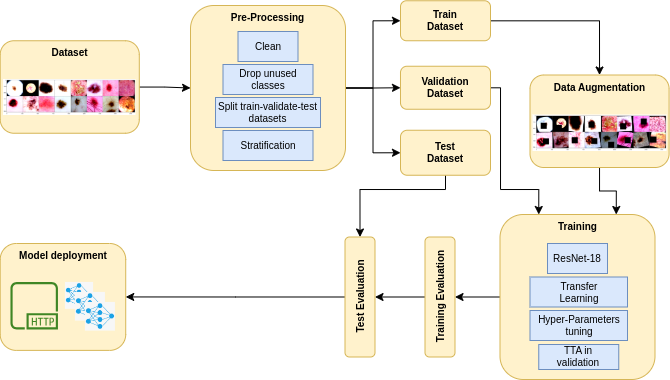
\includegraphics[width=\textwidth]{imatges/methodological_contribution/Pipeline.drawio.png}
%\end{adjustbox}
\caption[Training And Exposing CAD Infrastructure models]{\textit{Training And Exposing CAD Infrastructure models. Illustration by Author}}
{\label{fig:cad-infrastructure-training-system}}
\end{figure}

The first stage involves cleaning and splitting the initial dataset into smaller datasets. This step ensures that the data is organized and ready for further processing. \\

The second stage focuses on training and validating the models using the training and validation datasets. During this stage, the system reads images and applies data augmentation techniques to train images and Test Time Augmentation (TTA) to validation images. These techniques enhance the model's performance by introducing variations in the data and improving its generalization ability. \\

The third stage involves analyzing the training results obtained from different training approaches. In this section, we evaluate and analyze the model's performance by comparing the predicted results against the test dataset. This step helps us understand how well the models are learning and performing on unseen data. \\

The last stage revolves around exposing the trained models through an API's container image. This container image allows for easy deployment and integration of the models into other systems or applications, providing a convenient way to utilize the trained models for various tasks. \\

Overall, the pipeline depicted in \textit{Figure \ref{fig:cad-infrastructure-training-system}} showcases a systematic approach to training models, evaluating their performance, and making them available for consumption through an API infrastructure.
